\subsection{Patch}

\begin{frame}{Premiers patchs}
 \begin{figure}
   \caption{Programme sur bande perforée patchée pour Harvard Mark I.}
   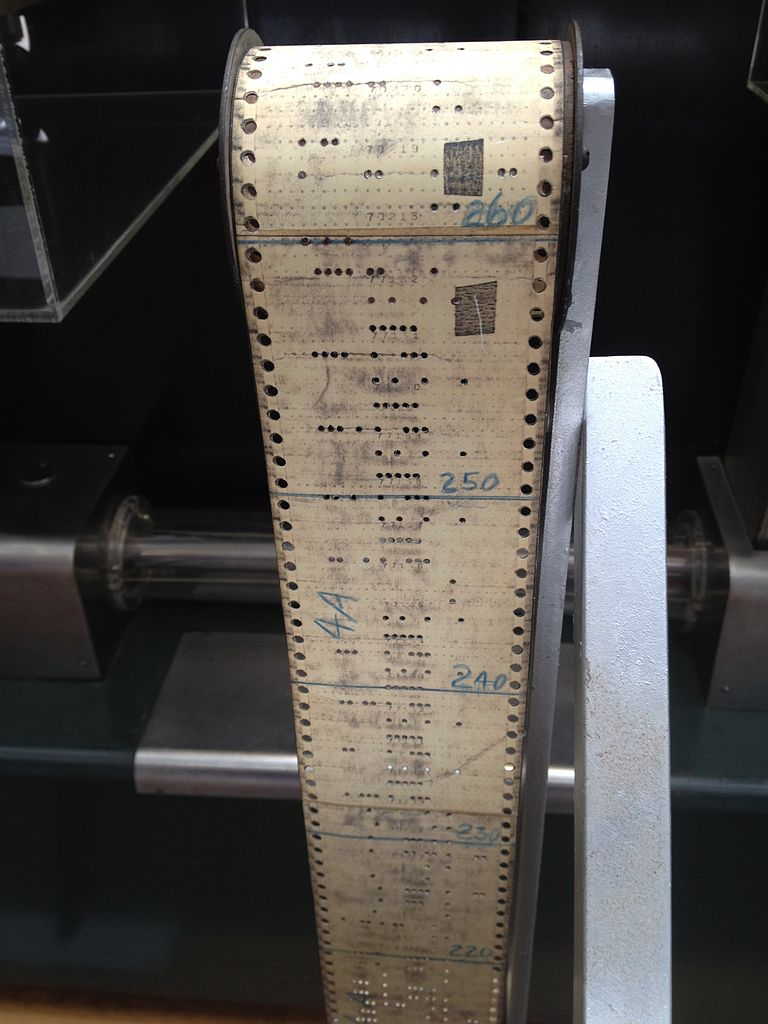
\includegraphics[height=160pt]{Harvard_Mark_I_program_tape}\par
   \tiny Source~: Wikipedia
 \end{figure}
\end{frame}

\begin{frame}[fragile]{Principe de base}
\begin{itemize}[<+->]
 \item Généralité~:
 \begin{itemize}
     \item Mécanisme permettant de modifier (correction, amélioration) une ressource.
  \end{itemize}
 \item Programmation~:
 \begin{itemize}[<+->]
    \item Fichier texte décrivant les différences entre deux fichiers texte~;
    \item Permet de stocker des incréments de modifications d'un fichier (révisions)~;
    \item Base de la gestion de versions.
  \end{itemize}
 \end{itemize}
\end{frame}

\begin{frame}[fragile]{Ligne de commande~: diff}
  \begin{itemize}[<+->]
  \item Commande de base permettant de comparer deux fichiers~:
  \begin{shell}
diff original.txt modifie.txt
  \end{shell}
  \item Series de ``morceaux'' (hunks)
  \begin{itemize}[<+->]
   \item Entête~: plages de lignes impactées et action~: \verb\ww[,yy]aWW[,YY]\~;
     \begin{description}[align=left]
      \item[a] add
      \pause
      \item[d] delete
      \pause
      \item[c] change (add and delete)
     \end{description}
   \item Lignes supprimées préfixées par \verb\<\~;
   \item Lignes ajoutées préfixées par \verb\>\~;
   \item Séparateur lorsque qu'il y a les deux (change)~: \verb\---\~;
   \item Dans le cas de plusieurs fichiers (\verb\-r\), la commande diff du fichier courant est ajoutée avant le premier morceau~: \verb\diff -r v1/fichier.txt v2/fichier.txt\~;
  \end{itemize}
  \item Possibilité d'avoir de la couleur avec \verb\colordiff\.
 \end{itemize}
\end{frame}

\begin{frame}[fragile]{Sortie normale de diff}
  \begin{tcbraster}[raster columns=3, raster valign=top]
  \begin{snvlisting}{original.txt}
This part of the
document has stayed the
same from version to
version.  It shouldn't
be shown if it doesn't
change.  Otherwise, that
would not be helping to
compress the size of the
changes.

This paragraph contains
text that is outdated.
It will be deleted in the
near future.

It is important to spell
check this dokument. On
the other hand, a
misspelled word isn't
the end of the world.
Nothing in the rest of
this paragraph needs to
be changed. Things can
be added after it.
  \end{snvlisting}
  \begin{snvlisting}{modifie.txt}
This is an important
notice! It should
therefore be located at
the beginning of this
document!

This part of the
document has stayed the
same from version to
version.  It shouldn't
be shown if it doesn't
change.  Otherwise, that
would not be helping to
compress anything.

It is important to spell
check this document. On
the other hand, a
misspelled word isn't
the end of the world.
Nothing in the rest of
this paragraph needs to
be changed. Things can
be added after it.

This paragraph contains
important new additions
to this document.
  \end{snvlisting}
  \begin{snvlisting}[[normal]diff]{diff original.txt modifie.txt}
0a1,6
> This is an important
> notice! It should
> therefore be located at
> the beginning of this
> document!
>
8,14c14
< compress the size of the
< changes.
<
< This paragraph contains
< text that is outdated.
< It will be deleted in the
< near future.
---
> compress anything.
17c17
< check this dokument. On
---
> check this document. On
24a25,28
>
> This paragraph contains
> important new additions
> to this document.
\end{snvlisting}
\end{tcbraster}
\end{frame}

\begin{frame}[fragile]{Script ed}
Format interprétable (presque) directement par la commande ed~:
\begin{shell}
printf "w\\nq\\n" >> v1v2.diff
ed -s original.txt < v1v2.diff
\end{shell}

\end{frame}

\begin{frame}[fragile]{Script ed}
\begin{tcbraster}[raster columns=3, raster valign=top]
  \begin{snvlisting}{original.txt}
This part of the
document has stayed the
same from version to
version.  It shouldn't
be shown if it doesn't
change.  Otherwise, that
would not be helping to
compress the size of the
changes.

This paragraph contains
text that is outdated.
It will be deleted in the
near future.

It is important to spell
check this dokument. On
the other hand, a
misspelled word isn't
the end of the world.
Nothing in the rest of
this paragraph needs to
be changed. Things can
be added after it.
  \end{snvlisting}
  \begin{snvlisting}{modifie.txt}
This is an important
notice! It should
therefore be located at
the beginning of this
document!

This part of the
document has stayed the
same from version to
version.  It shouldn't
be shown if it doesn't
change.  Otherwise, that
would not be helping to
compress anything.

It is important to spell
check this document. On
the other hand, a
misspelled word isn't
the end of the world.
Nothing in the rest of
this paragraph needs to
be changed. Things can
be added after it.

This paragraph contains
important new additions
to this document.
\end{snvlisting}
\begin{snvlisting}{diff -e original.txt modifie.txt}
24a

This paragraph contains
important new additions
to this document.
.
17c
check this document. On
.
8,14c
compress anything.
.
0a
This is an important
notice! It should
therefore be located at
the beginning of this
document!

.
\end{snvlisting}
\end{tcbraster}
\end{frame}

\begin{frame}[fragile]{Format contextuel}
\begin{itemize}[<+->]
 \item BSD 2.8 (Juillet 1981)~;
 \item Noms de fichiers et timestamp~;
 \item Lignes contexte~:
 \begin{itemize}[<+->]
  \item Lignes inchangées~;
  \item Préfixées par \textvisiblespace~;
  \item 3 par défaut~;
  \item Servent de référence pour valider la consistance du patch~;
  \item Permettent parfois de trouver l'emplacement du hunk lorsque les numéros de lignes sont changés dans le fichier sur lequel on applique le patch (fuzzy matching)~;
  \item Si lignes de contexte partagées entre deux parties modifiées, ces parties sont regroupées en un seul morceau.
 \end{itemize}
 \item Pas d'actions explicites, juste les préfixes \verb|-| (suppression), \verb|!| (modification) et \verb|+| (ajout)~;
 \end{itemize}
\end{frame}
 
\begin{frame}[fragile]{Format contextuel}
 \framesubtitle{Format d'un morceau}
 \begin{itemize}[<+->]
  \item Début~: \verb|***************|~;
  \item Plage de lignes concernées fichier source, encadrée par \verb|***|~;
  \item Contexte du début du morceau source, si pas au début du fichier~;
  \item Lignes supprimées (préfixées par \verb|-|), ou modifiées (préfixées par \verb|!|)~;
  \item Contexte de fin du morceau source, si pas en fin de fichier~;
  \item Plage de lignes concernées fichier cible, encadrée par \verb|---|~;
  \item Contexte du début du morceau cible, si pas au début du fichier~;
  \item Lignes ajoutées (préfixées par \verb|+|), ou modifiées (préfixées par \verb|!|)~;
  \item Contexte de fin du morceau cible, si pas en fin de fichier~;
 \end{itemize}
\end{frame}

\begin{frame}[fragile]{Format contextuel}
\begin{tcbraster}[raster columns=3, raster valign=top]
  \begin{snvlisting}{original.txt}
This part of the
document has stayed the
same from version to
version.  It shouldn't
be shown if it doesn't
change.  Otherwise, that
would not be helping to
compress the size of the
changes.

This paragraph contains
text that is outdated.
It will be deleted in the
near future.

It is important to spell
check this dokument. On
the other hand, a
misspelled word isn't
the end of the world.
Nothing in the rest of
this paragraph needs to
be changed. Things can
be added after it.
  \end{snvlisting}
  \begin{snvlisting}{modifie.txt}
This is an important
notice! It should
therefore be located at
the beginning of this
document!

This part of the
document has stayed the
same from version to
version.  It shouldn't
be shown if it doesn't
change.  Otherwise, that
would not be helping to
compress anything.

It is important to spell
check this document. On
the other hand, a
misspelled word isn't
the end of the world.
Nothing in the rest of
this paragraph needs to
be changed. Things can
be added after it.

This paragraph contains
important new additions
to this document.
\end{snvlisting}
\begin{snvlisting}[[context]diff]{diff -c original.txt modifie.txt}
*** original.txt	timestamp
--- modifie.txt	timestamp
***************
*** 1,3 ****
--- 1,9 ----
+ This is an important
+ notice! It should
+ therefore be located at
+ the beginning of this
+ document!
+
  This part of the
  document has stayed the
  same from version to
***************
*** 5,20 ****
  be shown if it doesn't
  change.  Otherwise, that
  would not be helping to
! compress the size of the
! changes.
!
! This paragraph contains
! text that is outdated.
! It will be deleted in the
! near future.

  It is important to spell
! check this dokument. On
  the other hand, a
  misspelled word isn't
  the end of the world.
--- 11,20 ----
  be shown if it doesn't
  change.  Otherwise, that
  would not be helping to
! compress anything.

  It is important to spell
! check this document. On
  the other hand, a
  misspelled word isn't
  the end of the world.
***************
*** 22,24 ****
--- 22,28 ----
  this paragraph needs to
  be changed. Things can
  be added after it.
+
+ This paragraph contains
+ important new additions
+ to this document.
\end{snvlisting}
\end{tcbraster}
\end{frame}

\begin{frame}[fragile]{Format unifié}
\begin{itemize}[<+->]
 \item Format développé en août 1990, ajouté à GNU diff 1.15 en janvier 1991~;
 \item Hérite des ajouts du format contextuel~:
 \begin{itemize}[<+->]
  \item Informations sur les fichiers~;
  \item Lignes de contexte.
 \end{itemize}
 \item Moins verbeux que le format contextuel car moins de répétitions~;
 \item Utilisé pour les échanges entre développeurs (notamment l'envoi par email).
\end{itemize}
\end{frame}

\begin{frame}[fragile]{Format unifié}
 \framesubtitle{Entête concernant le fichier impacté}
 \begin{itemize}[<+->]
  \item Fichier source préfixé par \verb|---| et timestamp de modification~;
  \item Fichier cible préfixé par \verb|+++| et timestamp de modification.
 \end{itemize}
\end{frame}

\begin{frame}[fragile]{Format unifié}
\framesubtitle{Format d'un morceau}
\begin{itemize}[<+->]
 \item Plages de lignes concernées~:
 \begin{itemize}[<+->]
   \item Chaque plage contient la ligne de début et la ligne de fin~;
   \item La plage côté source est préfixée par \verb|-|~;
   \item La plage côté cible est préfixée par \verb|+|~;
   \item Encadrées par \verb|@@|~;
   \item Optionnellement suivie d'un entête de section.
   \item \verb|@@ -l,s +l,s @@ optional section heading|
  \end{itemize}
  \item Contexte du début du morceau, si pas au début du fichier~;
  \item Lignes supprimées (préfixées par \verb|-|)~;
  \item Lignes ajoutées (préfixées par \verb|+|)~;
  \item Lignes modifiées : ajout et suppression~;
  \item Contexte de fin du morceau, si pas en fin de fichier~;
\end{itemize}
\end{frame}

\begin{frame}[fragile]{Format unifié}
\begin{tcbraster}[raster columns=3, raster valign=top, raster before skip=6pt]
  \begin{snvlisting}{original.txt}
This part of the
document has stayed the
same from version to
version.  It shouldn't
be shown if it doesn't
change.  Otherwise, that
would not be helping to
compress the size of the
changes.

This paragraph contains
text that is outdated.
It will be deleted in the
near future.

It is important to spell
check this dokument. On
the other hand, a
misspelled word isn't
the end of the world.
Nothing in the rest of
this paragraph needs to
be changed. Things can
be added after it.
  \end{snvlisting}
  \begin{snvlisting}{modifie.txt}
This is an important
notice! It should
therefore be located at
the beginning of this
document!

This part of the
document has stayed the
same from version to
version.  It shouldn't
be shown if it doesn't
change.  Otherwise, that
would not be helping to
compress anything.

It is important to spell
check this document. On
the other hand, a
misspelled word isn't
the end of the world.
Nothing in the rest of
this paragraph needs to
be changed. Things can
be added after it.

This paragraph contains
important new additions
to this document.
\end{snvlisting}
\begin{snvlisting}[[unified]diff]{diff -u original.txt modifie.txt}
--- original.txt   timestamp
+++ modifie.txt   timestamp
@@ -1,3 +1,9 @@
+This is an important
+notice! It should
+therefore be located at
+the beginning of this
+document!
+
 This part of the
 document has stayed the
 same from version to
@@ -5,16 +11,10 @@
 be shown if it doesn't
 change.  Otherwise, that
 would not be helping to
-compress the size of the
-changes.
-
-This paragraph contains
-text that is outdated.
-It will be deleted in the
-near future.
+compress anything.

 It is important to spell
-check this dokument. On
+check this document. On
 the other hand, a
 misspelled word isn't
 the end of the world.
@@ -22,3 +22,7 @@
 this paragraph needs to
 be changed. Things can
 be added after it.
+
+This paragraph contains
+important new additions
+to this document.
\end{snvlisting}
\end{tcbraster}
\end{frame}

\begin{frame}[fragile]{Application d'un patch}
\framesubtitle{Commande patch}
\begin{itemize}[<+->]
 \item Première version publié en 1985~:
 \begin{itemize}[<+->]
 \item Sur newsgroup \verb/mod.sources/ (devenu \verb/comp.sources.unix/)~;
 \item Par Larry Wall (créateur de Perl).
 \end{itemize}
 \item Version la plus utilisée~: GNU.
\end{itemize}
\end{frame}

\begin{frame}[fragile]{Commande patch}
\framesubtitle{Invocation}
 \begin{shell}
patch < v1v2.diff
 \end{shell}

 \begin{itemize}[<+->]
 \item Essaie de détecter le format parmis normal, script ed, contextuel ou unifié~;
 \item Se sert des informations de fichiers et de lignes dans le patch~;
 \item Si le patch n'est pas applicable directement, tente d'ignorer un certain nombre de lignes des contextes (fuzz factor, 2 par défaut)~;
 \item En cas de non application d'un morceau, il le met dans un fichier de rejet dont le nom est celui du fichier impacté suffixé par \verb|.rej|.
 \end{itemize}
\end{frame}
 
\begin{frame}[fragile]{Commande patch}
\framesubtitle{Options utiles}
\begin{itemize}[<+->]
 \item Forcer le format du patch~:
 \begin{itemize}[<+->]
  \item Normal~: \verb/-n/ ou \verb/--normal/~;
  \item Script ed~: \verb/-e/ ou \verb/--ed/~;
  \item Contextuel~: \verb/-c/ ou \verb/--context/~;
  \item Unifié~: \verb/-u/ ou \verb/--unified/.
 \end{itemize}
 \item Répertoire de travail~: \verb/-d/ ou \verb/--directory/~;
 \item Tronquer le début des chemins~: \verb/-p/num ou \verb/--strip=/num~: \verb/patch -p1 < v1v2.diff/
 \item Application inverse d'un patch (reverse, ou rollback)~: \verb/-R/ ou \verb/--reverse/~: \verb/patch -R < v1v2.diff/~;
 \item Suppression des fichiers vides après application du patch~: \verb/-E/ ou \verb/--remove-empty-files/~;
 \item Sauvegarde des fichiers originaux~: \verb/-b/ ou \verb/--backup/~;
% \item Mode bavard~: \verb/--verbose/.
\end{itemize}
\end{frame}

\begin{frame}[fragile]{Commande patch}
\framesubtitle{Exemples d'invocation}
\begin{tcbraster}[raster columns=2, raster valign=top]
\begin{snvlisting}[[unified]diff]{v1v2.diff}
diff -u v1/f1.txt v2/f1.txt
--- v1/f1.txt   2016-09-09 16:06:41.632285371 +0200
+++ v2/f1.txt   2016-09-09 16:07:12.913211867 +0200
@@ -1,3 +1,9 @@
+This is an important
+notice! It should
+therefore be located at
+the beginning of this
+document!
+
 This part of the
 document has stayed the
 same from version to
@@ -5,16 +11,10 @@
 be shown if it doesn't
 change.  Otherwise, that
 would not be helping to
-compress the size of the
-changes.
-
-This paragraph contains
-text that is outdated.
-It will be deleted in the
-near future.
+compress anything.

 It is important to spell
-check this dokument. On
+check this document. On
 the other hand, a
 misspelled word isn't
 the end of the world.
\end{snvlisting}
\begin{snvlisting}[[unified]diff]{}
@@ -22,3 +22,7 @@
 this paragraph needs to
 be changed. Things can
 be added after it.
+
+This paragraph contains
+important new additions
+to this document.
\end{snvlisting}
\end{tcbraster}
\end{frame}

\begin{frame}[fragile]{Commande patch}
\framesubtitle{Exemples d'invocation}
\begin{tcbraster}[raster columns=2, raster valign=top]
\begin{snvlisting}{Application réussie d'un patch}[][escapeinside={}]
# patch --verbose -p1 < v1v2.diff
Hmm...  Looks like a unified diff to me...
The text leading up to this was:
--------------------------
|diff -du v1/f1.txt v2/f1.txt
|--- v1/f1.txt  2016-09-11 16:06:41.632285371 +0200
|+++ v2/f1.txt  2016-09-11 16:07:12.913211867 +0200
--------------------------
patching file f1.txt
Using Plan A...
Hunk #1 succeeded at 1.
Hunk #2 succeeded at 11.
Hunk #3 succeeded at 22.
done
\end{snvlisting}
\begin{snvlisting}{Application échouée d'un patch}[][escapeinside={}]
# patch --verbose -p1 < v1v2.diff
Hmm...  Looks like a unified diff to me...
The text leading up to this was:
--------------------------
|diff -du v1/f1.txt v2/f1.txt
|--- v1/f1.txt  2016-09-11 16:06:41.632285371 +0200
|+++ v2/f1.txt  2016-09-11 16:07:12.913211867 +0200
--------------------------
patching file f1.txt
Using Plan A...
Reversed (or previously applied) patch detected!  Assume -R? [n] n
Apply anyway? [n] y
Hunk #1 FAILED at 1.
Hunk #2 FAILED at 5.
Hunk #3 FAILED at 22.
3 out of 3 hunks FAILED -- saving rejects to file f1.txt.rej
done
\end{snvlisting}
\end{tcbraster}
\end{frame}

\begin{frame}[fragile]{Commande patch}
\framesubtitle{Exemples d'invocation}
\begin{tcbraster}[raster columns=2, raster valign=top]
\begin{snvlisting}[[unified]diff]{f1.txt.rej}
--- f1.txt      2016-09-11 16:06:41.632285371 +0200
+++ f1.txt      2016-09-11 16:07:12.913211867 +0200
@@ -1,3 +1,9 @@
+This is an important
+notice! It should
+therefore be located at
+the beginning of this
+document!
+
 This part of the
 document has stayed the
 same from version to
@@ -5,16 +11,10 @@
 be shown if it doesn't
 change.  Otherwise, that
 would not be helping to
-compress the size of the
-changes.
-
-This paragraph contains
-text that is outdated.
-It will be deleted in the
-near future.
+compress anything.

 It is important to spell
-check this dokument. On
+check this document. On
 the other hand, a
 misspelled word isn't
 the end of the world.
\end{snvlisting}
\begin{snvlisting}[[unified]diff]{}
@@ -22,3 +22,7 @@
 this paragraph needs to
 be changed. Things can
 be added after it.
+
+This paragraph contains
+important new additions
+to this document.
\end{snvlisting}
\end{tcbraster}
\end{frame}

\begin{frame}[fragile]{Commande patch}
\framesubtitle{Exemples d'invocation}
 \begin{snvlisting}[[normal]diff]{diff ../v1v2.diff f1.txt.rej}
1,3c1,2
< diff -du v1/f1.txt v2/f1.txt
< --- v1/f1.txt 2016-09-11 16:06:41.632285371 +0200
< +++ v2/f1.txt 2016-09-11 16:07:12.913211867 +0200
---
> --- f1.txt    2016-09-11 16:06:41.632285371 +0200
> +++ f1.txt    2016-09-11 16:07:12.913211867 +0200
 \end{snvlisting}
\end{frame}

\begin{frame}[fragile]{Autres outils}
\framesubtitle{Merges avec diff3}
\begin{tcbraster}[raster columns=3, raster valign=top]
\begin{snvlisting}{diff3 -m v3/f1.txt v1/f1.txt v2/f1.txt}[][escapeinside={}]
This is an important
notice! It should
therefore be located at
the beginning of this
document!

This part of the
document has stayed the
same from version to
version.  It shouldn't
be shown if it doesn't
change.  Otherwise, that
would not be helping to
\end{snvlisting}
\begin{snvlisting}{}[][escapeinside={}]
<<<<<<< v3/f1.txt
compress the size of the
changes.

This paragraph contains
text that has been
modified on both sides.
It will be deleted in the
near future.
||||||| v1/f1.txt
compress the size of the
changes.

This paragraph contains
text that is outdated.
It will be deleted in the
near future.
=======
compress anything.
>>>>>>> v2/f1.txt
\end{snvlisting}
\begin{snvlisting}{}[][escapeinside={}]

It is important to spell
check this document. On
the other hand, a
misspelled word isn't
the end of the world.
Nothing in the rest of
this paragraph needs to
be changed. Things can
be added after it.

This paragraph contains
important new additions
to this document.
\end{snvlisting}
\end{tcbraster}
\end{frame}

\begin{frame}[fragile]{Autres outils}
\framesubtitle{Quilt}
\begin{itemize}[<+->]
 \item Nommé d'après patchwork quilt (courtepointe en patchwork)~;
 \item Permet de regrouper des ensembles de patchs en un seul~;
 \item Initialement développé par Andrew Morton, développeur Kernel Linux~;
 \item \url{https://stuff.mit.edu/afs/athena/system/i386_deb50/os/usr/share/doc/quilt/quilt.html}~;
 \item Très utilisé dans les projets Linux et Debian~;
 \item \url{https://wiki.debian.org/UsingQuilt}.
\end{itemize}
\end{frame}

%\begin{frame}{Cas pratiques}
%\framesubtitle{Paquet Debian : linux-image}
%\end{frame}